\documentclass[11pt]{report}

% Packages
\usepackage{graphicx}
\usepackage{algorithmicx}
\usepackage{algpseudocode}
\usepackage[linesnumbered,ruled,vlined]{algorithm2e}

% Page margins
\usepackage[margin=2.5cm]{geometry}

% Font
\usepackage{mathptmx}

% Title page
\title{\LARGE\bfseries\textbf{COMP9517: Computer Vision \\ 2023 Term 2 Assignment}}
\author{Zeal Liang\\z5325156}
\date{\today}
\begin{document}

\begin{titlepage}
  \centering
  
\includegraphics[width=0.8\textwidth]{Sydney Landscape.png}\par\vspace{1cm}
  {\scshape\LARGE University of New South Wales \par}
  \vspace{1cm}
  {\huge\bfseries COMP9517: Computer Vision\par}
  \vspace{1cm}
  {\huge\bfseries 2023 Term 2 Assignment\par}
  \vspace{2cm}
  {\Large\itshape Zeal Liang\\z5325156\par}
  \vfill
  % Bottom of the page
  {\large \today\par}
\end{titlepage}



\section*{Task 1: Otsu Thresholding}

In this task, I used the Otsu thresholding method for image binarization. Otsu thresholding is a method to automatically determine the threshold value and it selects the best threshold value by maximizing the inter-class variance for image segmentation.

The following are the methods and steps I used:

\begin{enumerate}
    \item Calculate and normalize the histogram: Since different images may have different number of pixels, the size of the histogram may also be different. In order to make the histograms of different sizes comparable with each other, we need to normalize them. Normalizing a histogram is the process of dividing each histogram entry by the total number of pixels so that each entry has a value between 0 and 1. This way, we can compare histograms of different sizes with each other without having to worry about their different sizes.
    \item Iteration over all thresholds: After initializing the variables for the best threshold and the maximum variance I iterate over all possible thresholds from 0 to 255.
    \item Calculating pixel probabilities and weights and means for class 1 and class 2: For each threshold, I calculate the probability and weight of pixels below the threshold as class 1, and the probability and weight of pixels above the threshold as class 2.
    \item Calculating inter-class variance: using the weights and means of class 1 and class 2, I calculated the inter-class variance. The between-class variance measures the degree of difference between the two categories, and a larger variance indicates a better segmentation of the categories. The formula for calculating the inter-class variance is given by:
    $$\sigma_{B}^{2}=p_{0}p_{1}(\mu_{0}-\mu_{1})^{2}$$
    \item Update the optimal threshold and maximum variance: If the current interclass variance is greater than the previous maximum variance, I update the maximum variance and set the current threshold to the optimal threshold.
    \item Apply optimal threshold: Based on the optimal threshold, I binarize the original image and set the pixels below the threshold to 0 (black) and the pixels above the threshold to 255 (white).
\end{enumerate}

\section*{Task 2: Isodata Thresholding}

In this task, I used Isodata thresholding method for image binarization. Isodata thresholding is an iterative based threshold selection method which minimizes the variance between two categories by continuously adjusting the threshold values.

The following are the methods and steps I used:

\begin{enumerate}
    \item Calculate and normalized histogram: same as \textbf{Task 1}
    \item Initialize variables: Initialize the threshold to 0 and set the new threshold to the histogram-weighted average.
    \item Convergence iteration: Enter the iteration process and stop iteration when the current threshold value and the new threshold value are the same. Otherwise, continue to the next step.
    \item Calculate the pixel probabilities and weights of class 1 and class 2: same as \textbf{Task 1}
    \item Calculate the mean value of class 1 and class 2: same as \textbf{Task 1}.
    \item Calculate the new threshold: By averaging the mean values of class 1 and class 2.
    \item Judging convergence: If the current threshold and the new threshold are the same, the convergence condition is reached and the iteration is stopped. Otherwise, continue to the next iteration.
    \item Apply the best threshold: same as \textbf{Task 1}
    \item The pseudo code is as follows

    \begin{algorithm}[H]
        \SetAlgoLined
        \KwIn{Image}
        \KwOut{Threshold}
        \SetKwFunction{FMain}{IsodataThresholding}
        \SetKwProg{Fn}{Function}{:}{}
        \Fn{\FMain{Image}}{
            \KwData{Select an arbitrary initial threshold $t$}
            \KwData{Compute $\mu_0$ and $\mu_1$ with respect to the threshold}
            \KwData{Update the threshold to the mean of the means: $t = (\mu_0 + \mu_1) / 2$}
            \While{the threshold changes}{
                \KwData{Compute $\mu_0$ and $\mu_1$ with respect to the threshold}
                \KwData{Update the threshold to the mean of the means: $t = (\mu_0 + \mu_1) / 2$}
            }
            \KwData{Upon convergence, the threshold is midway between the two class means}
            \KwRet{Threshold}
        }
        \caption{Isodata Thresholding}
    \end{algorithm}

\end{enumerate}


\section*{Task 3: Triangle Thresholding}

In this task, I used Triangle thresholding method for image binarization.The Triangle method is based on finding the threshold of the maximum distance which is the maximum distance between a straight line segment and the histogram distribution.

The following are the explanation and steps of the method:
\begin{enumerate}
    \item Find the highest or lowest gray level: Based on the peaks of the histogram, the highest or lowest gray level is determined. The location of the highest or lowest gray level is determined by comparing the number of pixels on either side of the peak.
    \item Calculate the slope and intercept of a straight line: Calculate the slope and intercept of a straight line using the number of pixels and the height between the peak and the highest gray level.
    \item Find the threshold for the maximum distance: traverse the pixel values of the histogram from the range between the highest gray level and the peak. For each pixel value, calculate the distance between the straight line and the histogram and find the threshold value that makes the distance maximum.
    \item Apply the best threshold: same as \textbf{Task 1}

    \item The pseudo code is as follows

    \begin{algorithm}[H]
        \SetKwFunction{GetGrayLevelPoint}{GetGrayLevelPoint}
        \KwIn{Histogram, Peak}
        \KwOut{GrayLevel}
        \SetKwProg{Fn}{Function}{:}{}
        \Fn{\GetGrayLevelPoint{hist, peak}}{
            \If{$\sum_{i=0}^{peak-1} hist[i] > \sum_{i=peak}^{255} hist[i]$}{
                \For{$i \gets 0$ \KwTo $255$}{
                    \If{$hist[i] \neq 0$}{
                        \KwRet $i$\;
                    }
                }
            }
            \Else{
                \For{$i \gets 255$ \KwTo $0$}{
                    \If{$hist[i] \neq 0$}{
                        \KwRet $i$\;
                    }
                }
            }
        }
        \caption{Find the highest or lowest gray level, depending on the peak}
    \end{algorithm}

    \begin{algorithm}[H]

        \SetAlgoLined
        \KwIn{Input image $I$}
        \KwOut{Automatically computed threshold value $T$}

        \SetKwFunction{Triangle}{Triangle}
        \SetKwProg{Fn}{Function}{:}{}
        \Fn{\Triangle{$I$}}{
            \KwData{Compute the histogram $H$ of image $I$ using the function $histogram(I)$\;}
            \KwData{Find the peak $(r_p, h_p)$ in histogram $H$ using the function $argmax(H)$\;}
            \KwData{Find the highest gray level point $(r_m, h_m)$ in histogram $H$ using the function $GetGrayLevelPoint(H, peak)$\;}
            \KwData{Construct a straight line $l(r)$ from $(r_p, h_p)$ to $(r_m, h_m)$\;}
            \KwData{Initialize the maximum distance $d_{max}$ to $-\infty$\;}
            \KwData{Initialize the threshold value $T$ to $0$\;}
            \For{each gray level $r$}{
                Compute the distance $d(r) = l(r) - h(r)$ using the function $distance(l(r), h(r))$\;
                \If{$d(r) > d_{max}$}{
                    Update $d_{max}$ to $d(r)$\;
                    Update $T$ to $r$\;
                }
            }
            \KwRet{$T$}\;
        }

        \KwRet{\Triangle{$I$}}\;
        \caption{Triangle Method for Threshold Computation}
    \end{algorithm}


\end{enumerate}


\section*{Task 4: Compare Thresholding Techniques}

    \subsection*{Differences in results and interpretation:}
    The Otsu method and the Isodata method performed basically the same in these five images. These two methods do not perform well in the Algae image. This may be because the distribution of gray levels is more concentrated in this plot and it is difficult to find a clear peak to determine the threshold.

    On the other hand the Triangle method performs poorly in the Nuclei and Rubik plots, although it has excellent performance in the Algae plot. This is because the Triangle method is based on the slope of the histogram and tries to find a "steep" region in the histogram and use it as a threshold for segmentation. This method is more suitable for images with a large concentration of pixel grayscale and is able to find the boundary between the foreground and the background more accurately.

    \subsection*{To summarize:}

        \begin{enumerate}
            \item Otsu method:
            It is suitable for images with significant gray level differences between the foreground and background. The Otsu method can provide accurate threshold segmentation when the distribution of gray levels in the image is relatively uniform or when there is an obvious bimodal distribution.

            \item Isodata method:
            It is suitable for images with a more uniform distribution of gray levels. When there is no significant gray level difference between foreground and background, Isodata method can provide better segmentation results.

            \item Triangle method:
            It is suitable for images with obvious boundaries and uneven distribution of gray levels. When there is a large asymmetry in the distribution of gray levels or an obvious single-peaked distribution, the Triangle method can accurately find the boundary between the foreground and the background.

        \end{enumerate}

    % Adjust table spacing
    \renewcommand{\arraystretch}{1.2}

    \begin{table}[htbp]
    \centering
    \resizebox{\textwidth}{!}{
        \begin{tabular}{|c|c|c|c|c|}
        \hline
        \textbf{\huge Original Image}                       & \textbf{\huge Histogram}                        & \textbf{\huge Otsu}                             & \textbf{\huge Isodata}                             & \textbf{\huge Triangle}                             \\
        \hline
        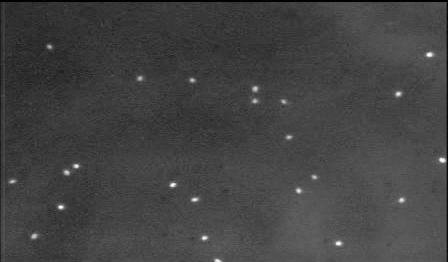
\includegraphics[width=5cm]{Algae.png}     & 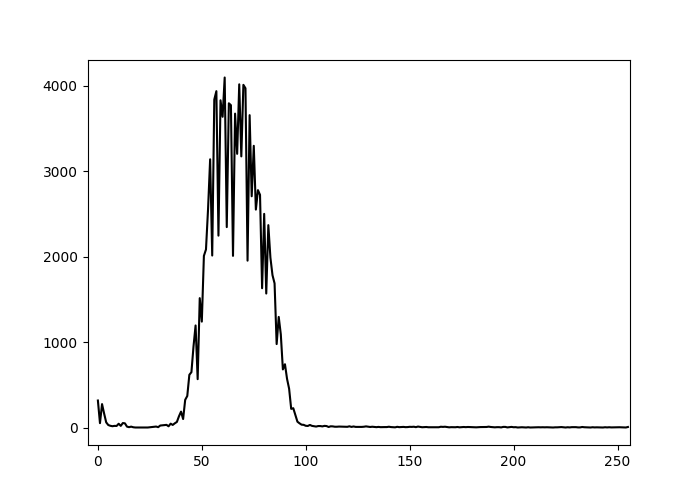
\includegraphics[width=5cm]{Algae_Hist.png}     & 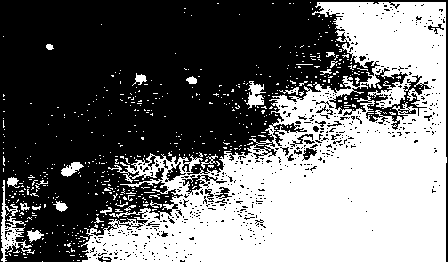
\includegraphics[width=5cm]{Algae_Otsu.png}     & 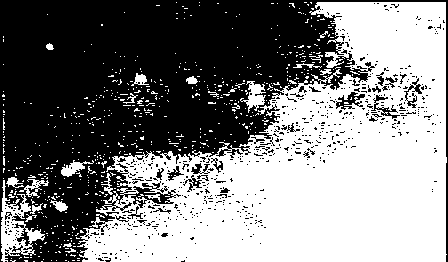
\includegraphics[width=5cm]{Algae_Isodata.png}     & 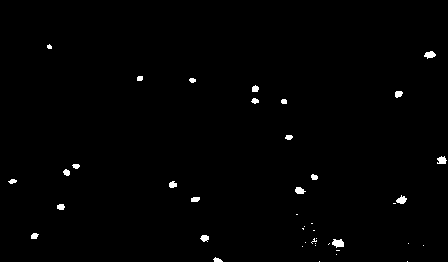
\includegraphics[width=5cm]{Algae_Triangle.png}     \\
        \hline
        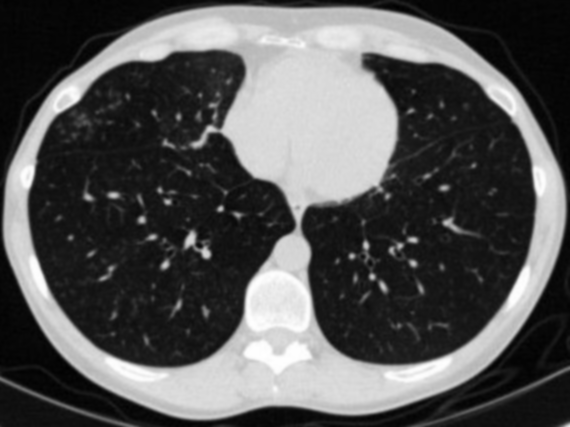
\includegraphics[width=5cm]{CT.png}        & 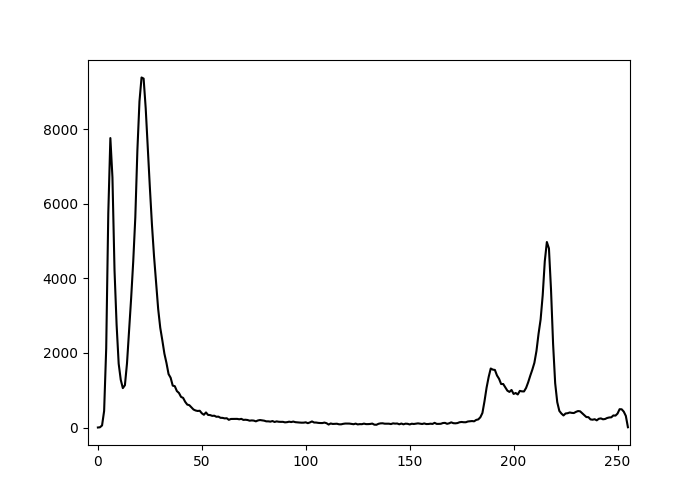
\includegraphics[width=5cm]{CT_Hist.png}        & 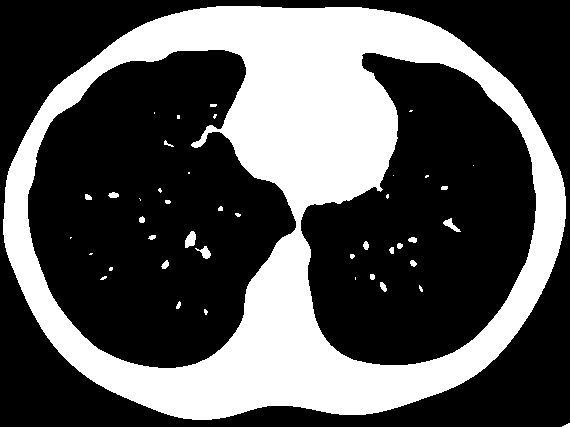
\includegraphics[width=5cm]{CT_Otsu.png}        & 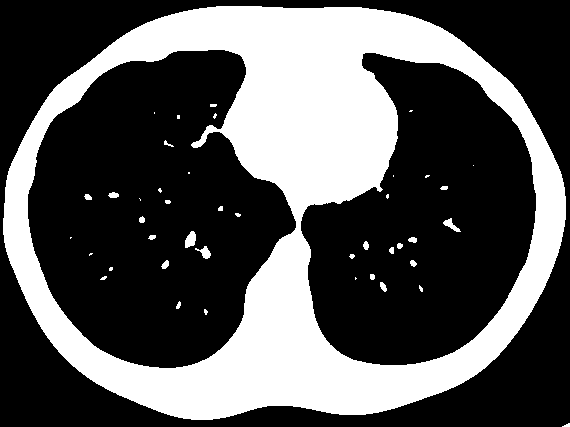
\includegraphics[width=5cm]{CT_Isodata.png}        & 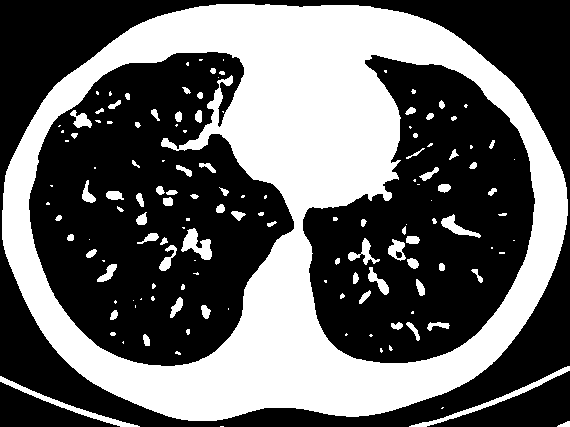
\includegraphics[width=5cm]{CT_Triangle.png}        \\
        \hline
        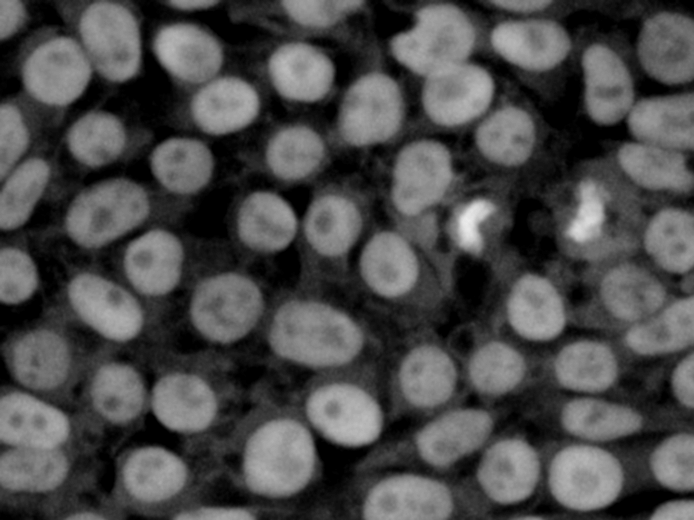
\includegraphics[width=5cm]{Nuclei.png}    & 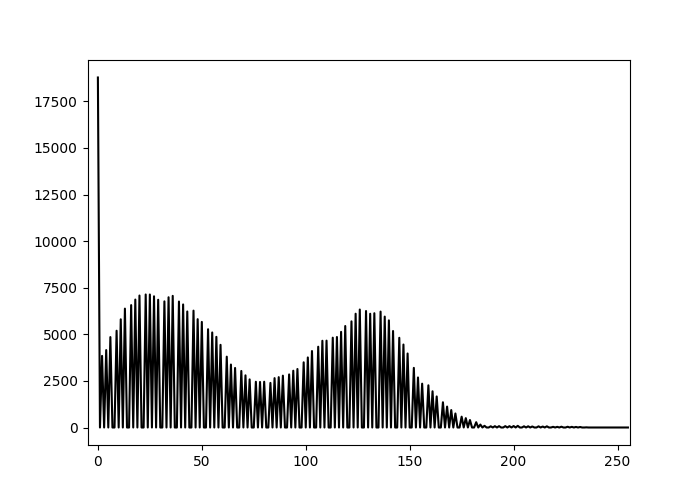
\includegraphics[width=5cm]{Nuclei_Hist.png}    & 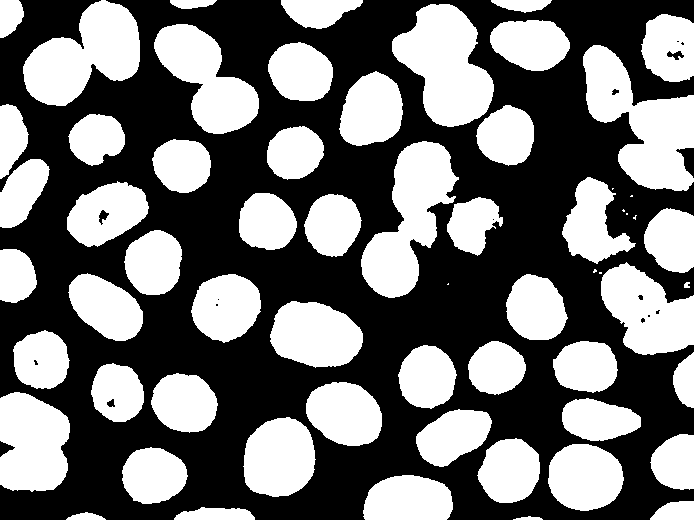
\includegraphics[width=5cm]{Nuclei_Otsu.png}    & 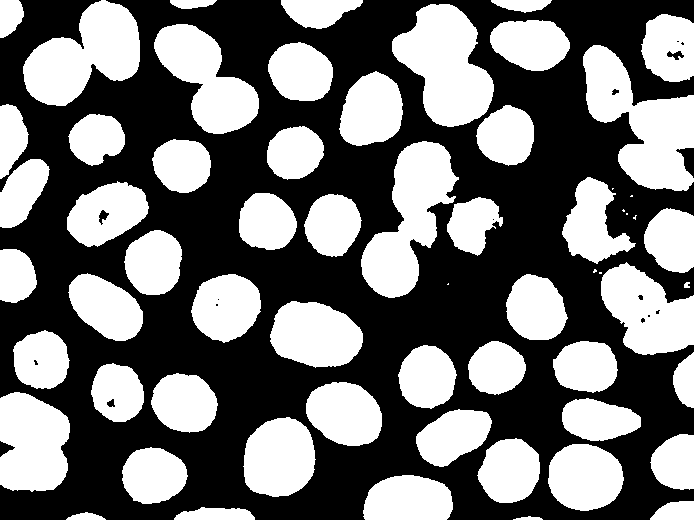
\includegraphics[width=5cm]{Nuclei_Isodata.png}    & 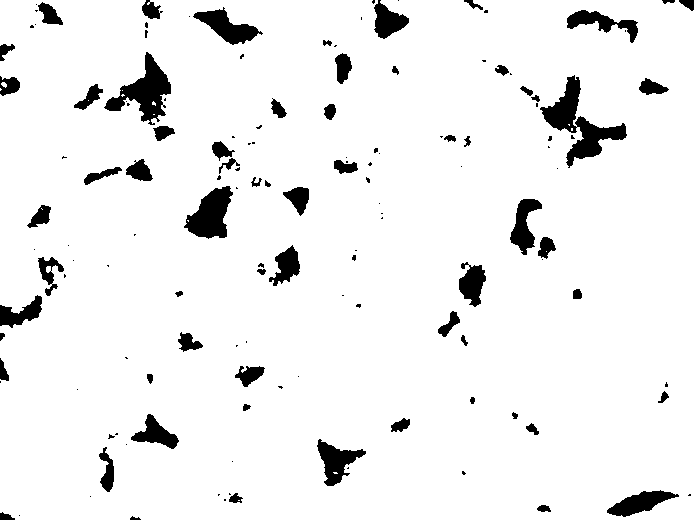
\includegraphics[width=5cm]{Nuclei_Triangle.png}    \\
        \hline
        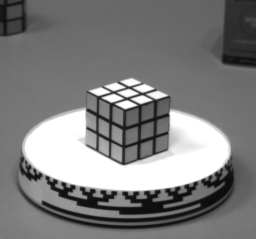
\includegraphics[width=5cm]{Rubik.png}     & 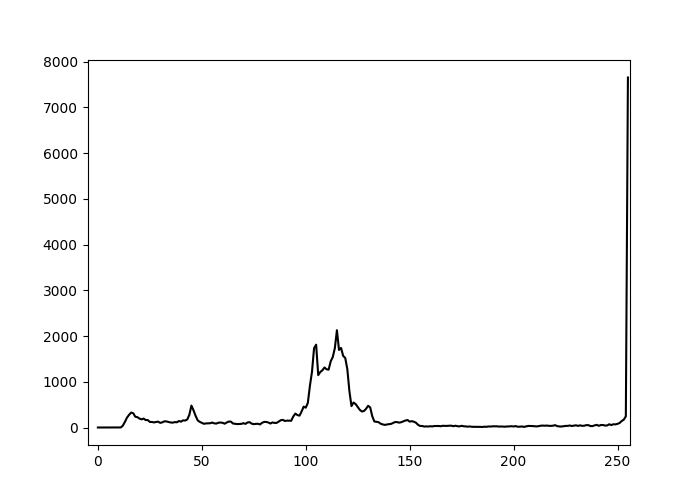
\includegraphics[width=5cm]{Rubik_Hist.png}     & 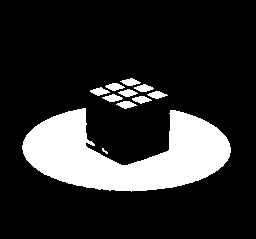
\includegraphics[width=5cm]{Rubik_Otsu.png}     & 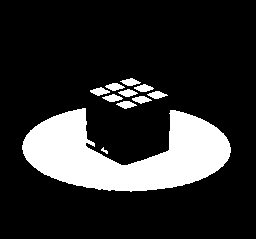
\includegraphics[width=5cm]{Rubik_Isodata.png}     & 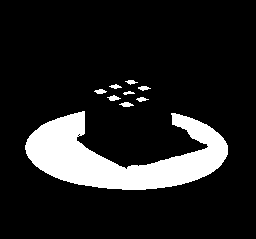
\includegraphics[width=5cm]{Rubik_Triangle.png}     \\
        \hline
        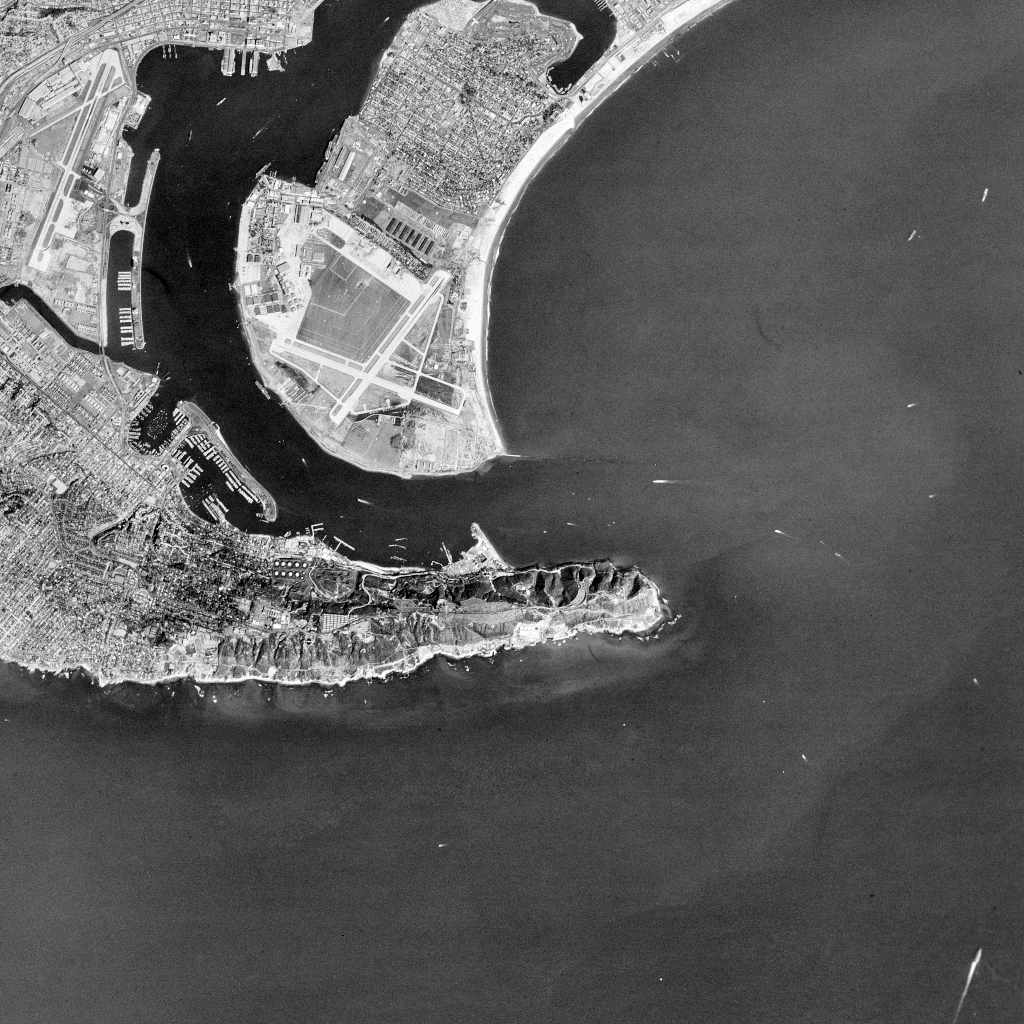
\includegraphics[width=5cm]{Satellite.png} & 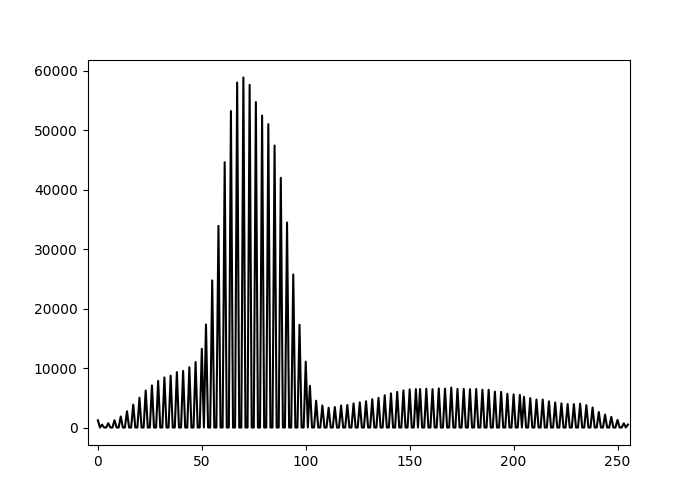
\includegraphics[width=5cm]{Satellite_Hist.png} & 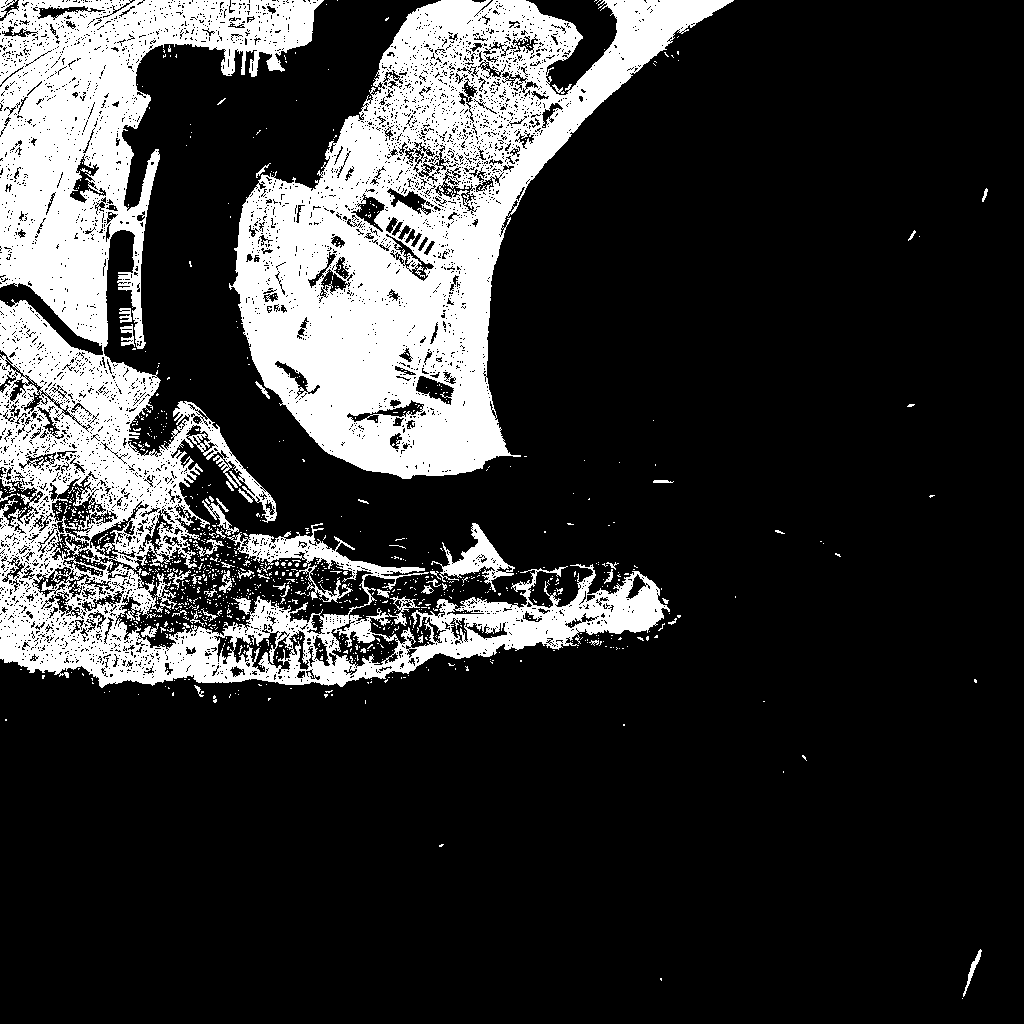
\includegraphics[width=5cm]{Satellite_Otsu.png} & 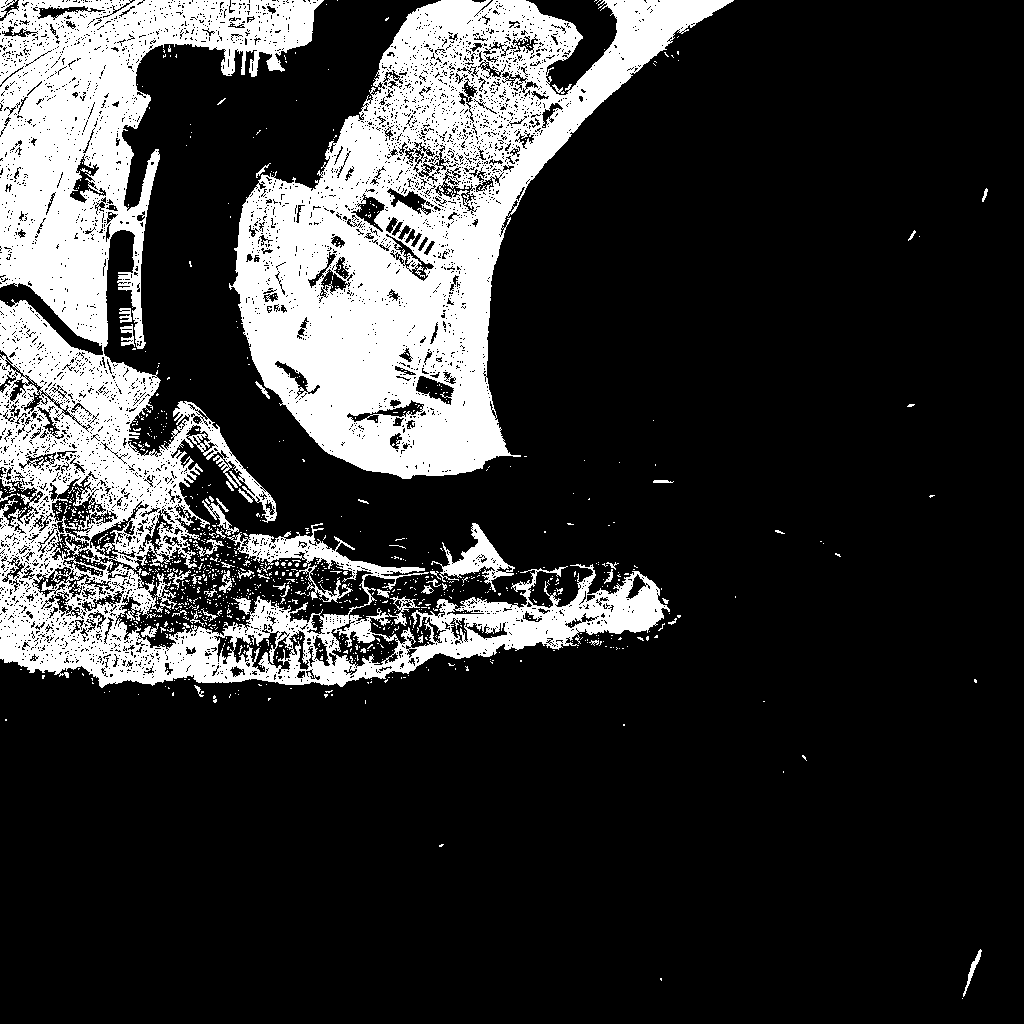
\includegraphics[width=5cm]{Satellite_Isodata.png} & 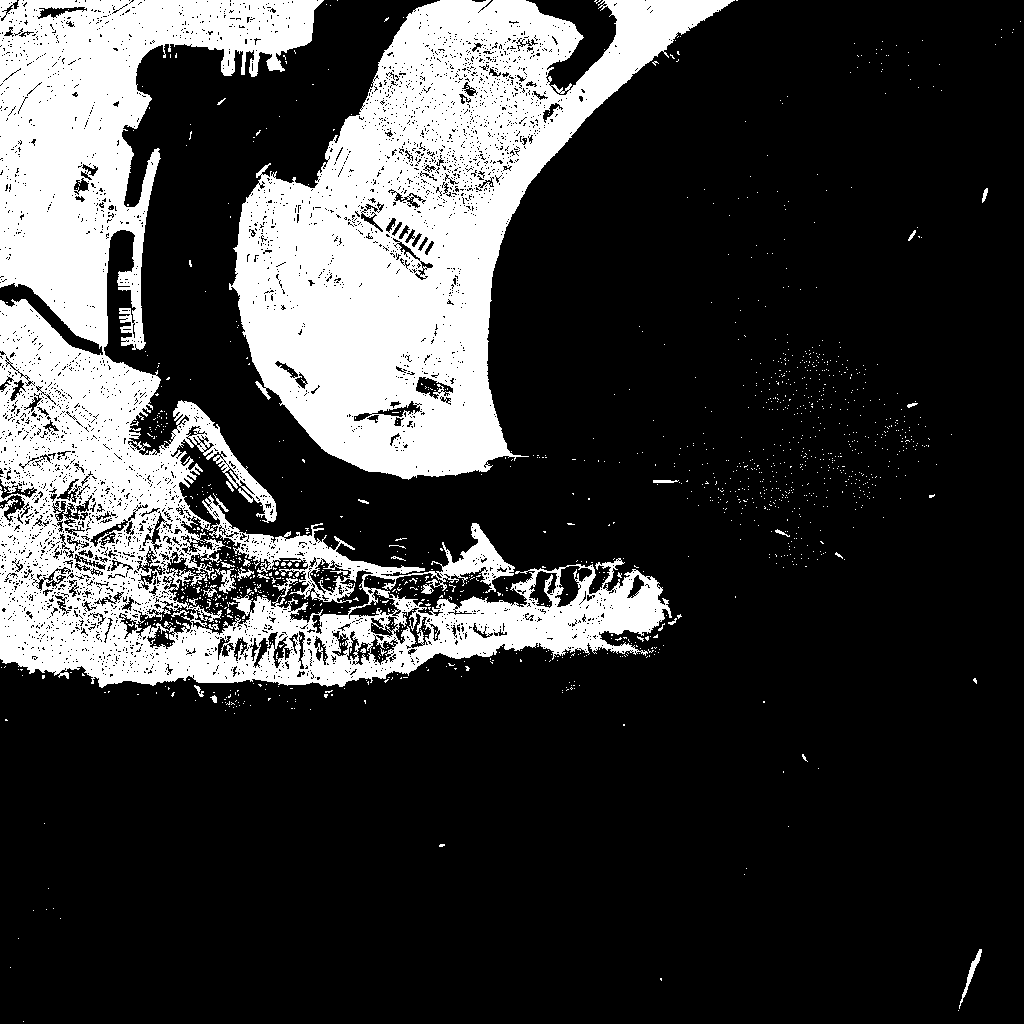
\includegraphics[width=5cm]{Satellite_Triangle.png} \\
        \hline
        \end{tabular}%
    }
    \caption{Comparison of different thresholding methods on various images.}
    \label{tab:thresholding_comparison}
    \end{table}

\end{document}

